\documentclass[12pt, a4paper]{article}
\usepackage[margin=3cm, top=3cm]{geometry}
\usepackage{tocloft}
\usepackage{graphicx}
\usepackage{makecell}
\usepackage{ragged2e}



\usepackage{lipsum}  % Package for generating dummy text

% CONSTANTS
%----------------------------------------
\newcommand{\gametitle}{Flee or Freeze}
\newcommand{\gamedevs}{Menoukagyuu}
\newcommand{\gameartist}{}
\newcommand{\gamemusician}{}
%----------------------------------------


\title{\gametitle}

\begin{document}
{ % Head
    {
        \titlepage{
            {
                \Huge
                \begin{center}
                    \textbf{\gametitle\\Game Design Document\\
                        {
                            \normalsize
                            For the ''\textit{Nokia 3310 Game Jam 6}''
                        }
                    }
                \end{center}
            }
        
            \hrule
            {
                \large
                \tableofcontents
            }
        }
    }\newpage

    \section{Introduction}
        In \textbf{\gametitle} you are imprisoned by the local magical police department
        and your goal is to escape it without beeing seen.
        
        \subsection{Game Summary}
            You have been captured while fighting your arch enemy on the street.
            But when the MPD arraived he somehow convinced them that you are the
            aggressor. So the MPD freezes you in time and take you to their
            police department for further investigations. You know that
            the cards are against you in this situation, so you make the 
            decision to flee the prison that holds you.

        \subsection{Inspiration}
            \textbf{Robbery Bob}: A comic styled robbery game where you have to steal
            as much as you can without getting seen by the local inhabitants and security.
            \begin{figure}[h]
                \centering
                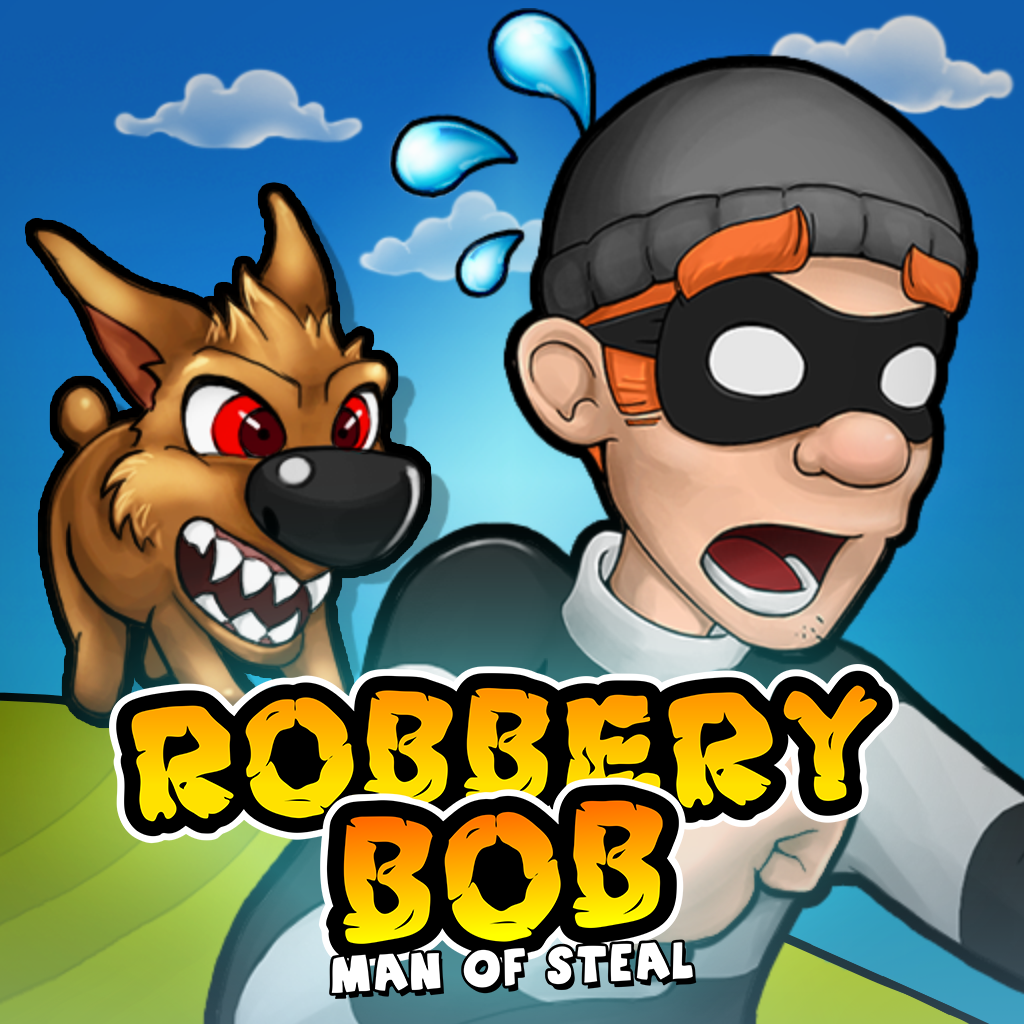
\includegraphics[scale=0.15]{./images/robberybob.png}
            \end{figure}

        \subsection{Player Experience}
            In a scrolling screen area a player has to reach the goal while also
            avoiding the sight of NPCs. With increasing difficulties.
            The Player can also upgrade himself before each game run by 
            buying upgrades or tools from an NPC in the prison.

        \subsection{Platform}
            The game is developed on linux but with releases for windows and linux.

        \subsection{Development Software}
            \begin{table}[h]
                \begin{tabular}{| l | l |}\hline
                    \textbf{Game Programming} &  \thead{The Game programming is done in the \textit{Godot Game Engine}}\\\hline
                    \textbf{Art} & The art is done in \textit{Aseprite}\\\hline
                    \textbf{Music} & The music is done in \textit{Reaper DAW}\\\hline
                \end{tabular}
            \end{table}

        \subsection{Genre}
            Hide and seek, Pixel Art, Escape, casual

        \subsection{Target Audience}
            The target audience are players who search for a
            stealth game with ingreasing difficulties.

    \section{Concept}

        \subsection{Gameplay overview}
            The player controlls a person which tries to escape a situation
            therefor it can sneek, walk, and sprint, all movement abillities
            have got an incremental sound pollution which will alarm surounding guards.
            By using the envoironment, like a wall or a mooving vehicle, the player tries
            to stay out of sight for the guards. Additionally while progressing
            througout the game, the player can get power ups which makes it move
            faster without makeing more noise or use magic powers to create a 
            distraction.

        \subsection{Theme Interpretation} % Only for game jams
            When the player gets caugth the guards use a freezing spell
            to freeze the player in time and take it back to the prison cell.

        \subsection{Primary Mechanics}
            \begin{table}[h]
                \centering
                \begin{tabular}{| m{7cm} | m{7cm} |}\hline
                    \thead{\textbf{Movement}\\The Player can either sneek, \\walk or sprint. These forms offer \\a variety between speed and stealthness} & Pic\\\hline
                    \thead{\textbf{Guards}\\The Guards are looking out for the Player\\In early levels they are very passive\\but later they will actively \\search for the player} & Pic\\\hline
                \end{tabular}
            \end{table}
        \newpage
        \subsection{Secondary Mechanics}
            \begin{table}[h]
                \centering
                \begin{tabular}{| m{7cm} | m{7cm} |}\hline
                    \thead{\textbf{Moving Objcects}\\From time to time there is an\\oportunity to use a moving\\object to cross an unsafe area} & Pic\\\hline
                    \thead{\textbf{Distraction}\\Later in game the player\\will be able to generate\\distractions for the guards by\\using magic} & Pic\\\hline
                \end{tabular}
            \end{table}
    \section{Art}
        
        \begin{figure}[h]
            \centering
            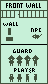
\includegraphics[scale=2]{./images/concept.png}
        \end{figure}

        \subsection{Theme Interpretation} % Only for game jams
            The Game art is based on the old Nokia 3310 graphics.
            The color pallet is fixed by the following one.
            \begin{figure}[h]
                \centering
                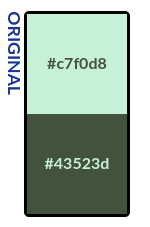
\includegraphics[scale=0.7, angle=90]{./images/colorpallet.png}
            \end{figure} 

        \subsection{Design}
            Because of the main theme of this Game Jam the color 
            pallet and the screen resolution, 84 x 48 pixel, is very limited.
            So the Design of the game graphics will be very simple and sharp.

    \section{Audio}

        \subsection{Music}
            To add a nostalgic fealing to the game, only the old Nokia 3310
            sounds will be used. Non then less should the music be mysterious
            and threatening to give the player a fealing of an intense 
            situation for a more immersive experience.

        \subsection{Sound Effects}
            Sound effects are rearly used because the nokia 3310
            has got only one audio chanell. Therefore the music 
            allways needs to be take a break when playing a sound
            effect. Possible situations are, when the player was very noisy
            and the guards are alarmed of the presence of the player. Also
            the distraction action could get a sound effect.

    \section{Game Experience}
    
        \subsection{UI}
            The games UI is weaved together with the prison cell,
            where different places lets the player access different
            options. Like the store NPC, Settings on a wall board.
            
        \subsection{Controls}
            The Player Movement will be controlled by either numpad (8 4 2 6)
            or by the std keys (W A S D). Additionally the player can use the (7/Q)
            Keys to change the walking speed, and the (9/E) Key for abillities.

    \section{Development Timeline}
        \begin{table}[h]
            \centering
            \begin{tabular}{| m{4cm} | m{4cm} | m{4cm}|}\hline
                \textbf{Task} & \textbf{Status} & \textbf{Date}\\\hline\hline
                Creating Art & Done & 18.02.2024\\\hline
                Creating Music & Done & 18.02.2024\\\hline
                Creating Sound effects & WIP &\\\hline
                Game Programming  &  & \\\hline
                Testing & & \\\hline
                Realease & & \\\hline
            \end{tabular}
        \end{table}
}

\end{document}